\chapter{Analisi e Progettazione}
Come anticipato nel capitolo introduttivo, il progetto prevede la creazione di un'aula virtuale in cui il docente e gli studenti possono comunicare tra loro e interagire con l'ambiente circostante.
\\In questo capitolo verrà illustrata prima la fase di analisi, attraverso la specifica dei requisiti e dei casi d'uso, successivamente la fase di progettazione, con i diagrammi di \textbf{\textit{workflow}} (flussi di lavoro).
\section{Specifica dei Requisiti}
L'analisi dei requisiti funzionali, ha fatto emergere alcune delle proprietà che il sistema deve necessariamente avere per soddisfare la richiesta.
\\La prima proprietà riguarda gli attori del sistema, secondo la specifica, infatti, è necessario
distinguere due attori:
\begin{itemize}
    \item Docente
    \item Studente
\end{itemize} 
Questa distinzione implica la necessità di introdurre un sistema di autenticazione
in modo tale da poter identificare l'utente e il suo ruolo all'interno
dell'applicazione.\\
Una seconda proprietà emersa riguarda il tipo di interazioni che gli attori
possono avere tra loro, perciò è stato introdotto un mezzo di comunicazione fra utenti connessi.
\\Infine, è stato necessario introdurre un sistema che permettesse agli utenti
di interagire con l'ambiente circostante, in particolare il docente deve avere la
possibilità di indicare un punto di interesse all'interno della scena virtuale.\\
Questa breve descrizione delle funzionalità richieste ci permette di identificare
più in dettaglio i requisiti funzionali:
\begin{itemize}
    \item Il sistema deve permettere l'identificazione dell'utente, in modo da poterne
     stabilire il ruolo; 
     \item Il sistema deve consentire agli attori di accedere ad uno spazio comune e
di potersi vedere reciprocamente;
     \item All'interno dello spazio comune il sistema deve fornire uno strumento di
comunicazione agli utenti;
     \item All'interno dello spazio comune il sistema deve prevedere la possibilità, da
parte del docente, di indicare un punto di interesse.
\end{itemize} 
Un forte vincolo imposto all'applicazione è rappresentato dall'assenza di un'iscrizione o registrazione.\\ Per semplicità, si è deciso di trascurare questa funzionalità aggiuntiva che necessiterebbe di un \gls{database}, per memorizzare i dati di accesso degli utenti, e di una funzionalità per l'accesso ai dati.
\\Le credenziali di autenticazione sono specificate in un file json.
\section{Analisi dei casi d'uso}
La specifica dei requisiti indica chiaramente la presenza di due attori che
condividono alcune funzionalità comuni, pertanto è stata creata una generalizzazione,
chiamata User, di questi due attori.
\\Per questo motivo, è previsto un sistema di autenticazione che distingue il ruolo dello studente da quello del docente.
\begin{figure}[H]
    \centering
    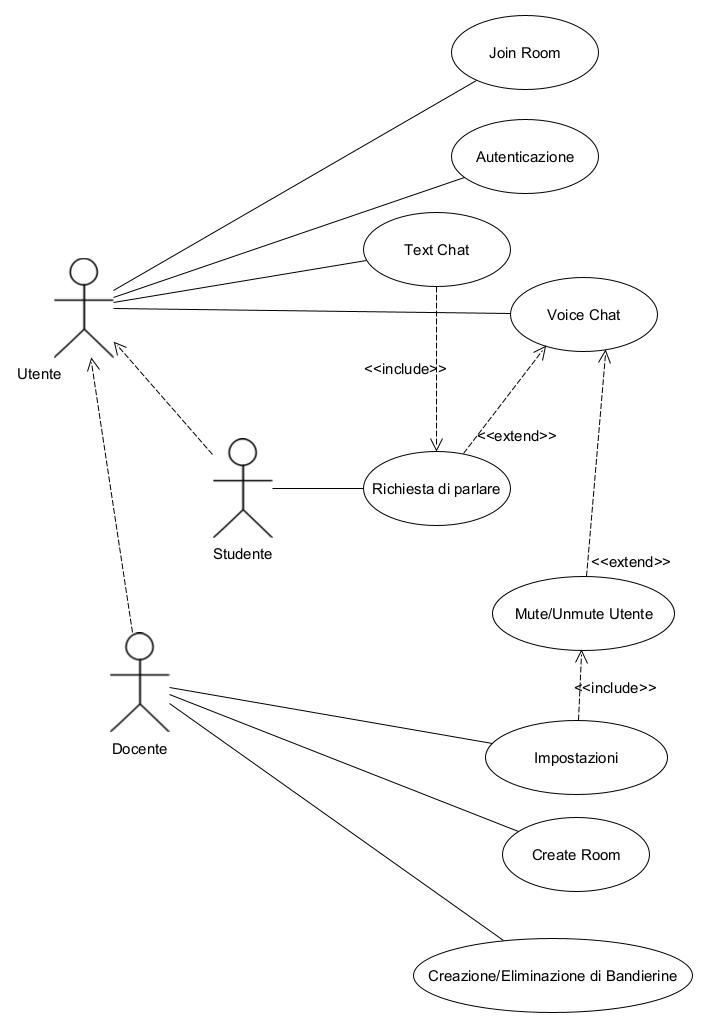
\includegraphics[width = 13cm, height = 16cm]{Immagini/AppUseCase (complete).jpg}
    \caption{Diagramma completo dei casi d'uso }
    \label{fig:my_label}
\end{figure} 
\hspace*{-0.6cm}Dalle specifiche dei requisiti sono stati identificati 7 casi d'uso, ovvero la descrizione di un insieme di interazioni, tra un utente ed un sistema, che consentono all'utente di raggiungere un obiettivo o di svolgere un compito:
\begin{itemize}
\item Autenticazione;
\item Create Room;
\item Join Room;
\item Chat Vocale;
\item Chat di testo;
\item Richiesta di parlare;
\item Impostazioni;
\item Mute/Unmute Utente;
\item Creazione/Eliminazione di bandierine.
\end{itemize}
\subsection{Autenticazione}
Dalle specifiche risulta evidente  la  necessità  di  distinguere  gli  utenti  in  due  attori, perciò è stato introdotto un meccanismo di autenticazione necessario per la verifica dell'identità dell'utente.
\\Il caso d'uso \textit{Autenticazione} inizia in seguito all'avvio dell'applicazione, dopodiché l'attore inserisce le proprie credenziali, ovvero \textit{username} e \textit{password} e clicca sul bottone \textit{login}.
\\Se le credenziali sono errate, il sistema mostrerà un messaggio di errore, se invece l'autenticazione ha successo, l'attore verrà indirizzato verso una nuova scena che differisce a seconda del ruolo in cui si è identificato.
\begin{figure}[H]
    \centering
    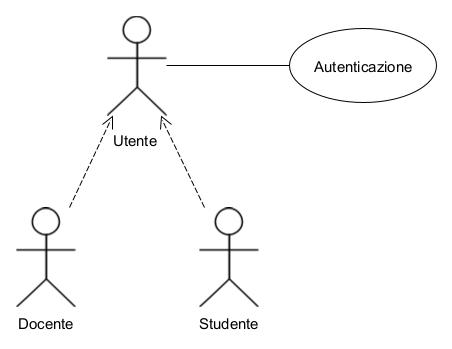
\includegraphics[scale=0.5]{Immagini/LoginUseCase.jpg}
    \caption{Diagramma del caso d'uso Autenticazione}
    \label{fig:my_label}
\end{figure}
\subsection{Create Room}
Il caso d'uso \textit{Create Room} ha come precondizione aver effettuato l'autenticazione con successo con il ruolo di docente.
\\Il sistema mostra all'attore una schermata con la lista delle aule già create, se presenti, e offre la possibilità di creare una nuova aula, assegnandole un nome. \\In seguito alla creazione della stanza, il docente viene automaticamente indirizzato alla scena relativa all'aula appena creata.\\Pertanto, sia che il docente crei una nuova stanza oppure scelga di entrare in un'aula già presente, il sistema caricherà la scena corretta per l'attore.
\subsection{Join Room}
\begin{figure}[H]
    \centering
    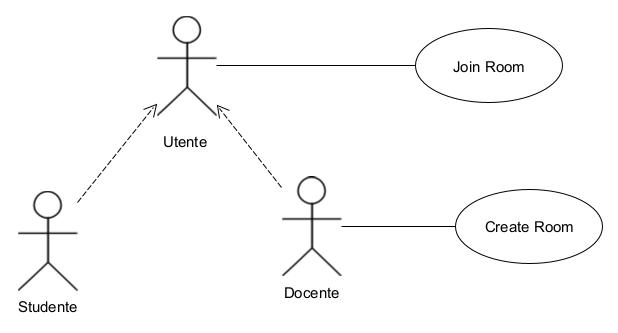
\includegraphics[scale=0.6]{Immagini/CreateJoinRoomUseCase.jpg}
    \caption{Diagramma dei caso d'uso Join Room e Create Room}
    \label{fig:my_label}
\end{figure}
Il caso d'uso \textit{Join Room} ha come precondizione aver effettuato l'autenticazione con successo con uno dei ruoli resi a disposizione dal sistema.
\\Il sistema presenta una schermata in cui viene mostrato l'elenco delle aule già disponibili. \\L'utente può scegliere tra le aule presenti ed entrare in una di queste, cliccando direttamente sul nome dell'aula.
\\Nel caso di un docente, l'ingresso in una stanza verrà effettuato non solo attraverso la scelta tra quelle disponibili, ma anche dopo aver effettuato la creazione di una nuova stanza.
\subsection{Chat Vocale}
Il caso d'uso \textit{Chat Vocale} ha come precondizione l'accesso ad uno spazio condiviso da due o più utenti. \\In questa fase non sono richieste particolari azioni da parte degli attori, ma risulta importante evidenziare come essi ottengano valore da questo caso d'uso, infatti è da questo che gli utenti ottengono la possibilità di comunicare tra loro tramite i microfoni e le cuffie.
\\Non appena gli attori accedono alla stessa aula, il sistema permette loro di comunicare e di vivere un'esperienza audio realistica attraverso la tecnologia \textbf{audio 3D}, che consente all'ascoltatore di percepire il suono da ogni direzione.
\subsection{Chat di testo}
Il caso d'uso \textit{Chat di testo} ha come precondizione l'accesso ad uno spazio condiviso da due o più utenti.
\\Il sistema garantisce una comunicazione network attraverso una interfaccia utente nella quale è possibile scrivere dei messaggi e inviarli agli altri utenti.
\subsection{Richiesta di parlare} \label{Request}
\begin{figure}[H]
    \centering
    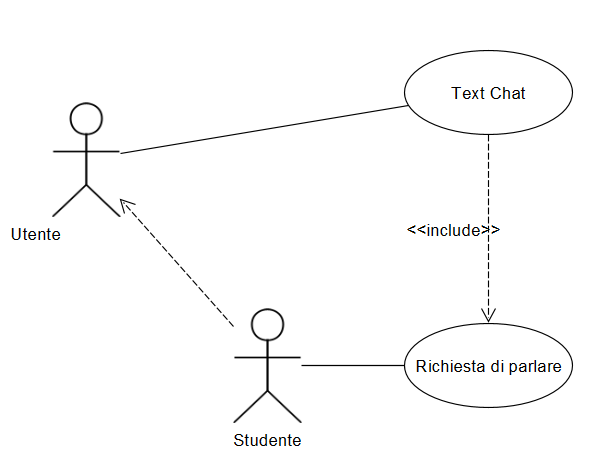
\includegraphics[scale=0.6]{Immagini/text.jpg}
    \caption{Diagramma del caso d'uso Text Chat che include Richiesta di Parlare}
    \label{fig:my_label}
\end{figure}
Il caso d'uso \textit{Richiesta di Parlare} ha come precondizione l'accesso ad uno spazio condiviso da due o più utenti e che l'attore di questo caso d'uso abbia il ruolo di studente.
\\Come detto in precedenza, all'interno dell'aula, il docente avrà l'autorità di concedere la parola ad uno studente, a tutti, oppure togliere questo diritto a sua discrezione. \\Questo potrebbe portare ad una comunicazione unilaterale in cui gli studenti sono attori passivi della comunicazione. \\Per ovviare a questo possibile inconveniente, gli studenti hanno la possibilità di richiedere la parola. \\Per fare ciò, nella schermata della chat di testo presentata dal sistema, sarà presente un bottone che invierà sulla chat una notifica, della forma: \textit{`Nome studente} richiede di parlare`, a tutti gli utenti. \\A questo punto il docente può decidere se concedere la parola allo studente che l'ha richiesta.
\subsection{Impostazioni}
Il caso d'uso \textit{Impostazioni} ha come precondizione l'accesso ad uno spazio condiviso da due o più utenti e che l'attore di questo caso d'uso abbia il ruolo di docente.
\\Il sistema mostrerà al docente una schermata, che possiede l'elenco dei nomi dei giocatori connessi alla stanza, nella quale sono abilitate le funzioni del caso d'uso \textit{Mute/Unmute Utente}.
\subsection{Mute/Unmute Utente}
Il caso d'uso \textit{Mute/Unmute Utente} ha come precondizione l'accesso ad un'aula da parte di più utenti e che l'attore di questo caso d'uso abbia il ruolo di docente. \\All'interno dell'aula, il docente avrà l'autorità di concedere la parola ad uno studente, a tutti, oppure togliere questo diritto a sua discrezione. \\Il docente avrà la possibilità di vedere l'elenco degli studenti presenti nell'aula e, accanto ai loro nomi, sarà presente un bottone che permetterà di dare e togliere la parola al relativo studente.
\begin{figure}[H]
    \centering
    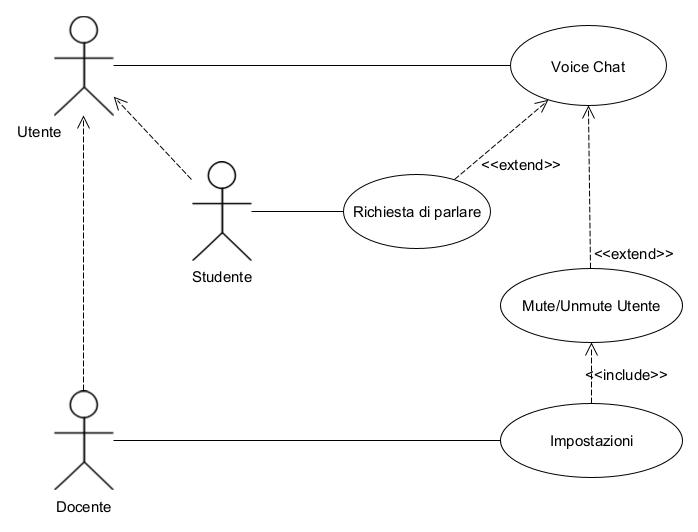
\includegraphics[scale=0.6]{Immagini/VoiceChatUseCase.jpg}
    \caption{Diagramma dei caso d'uso Voice Chat, Mute/Unmute Utente, Impostazioni}
    \label{fig:my_label}
\end{figure}
\subsection{Creazione/Eliminazione di bandierine}
Il caso d'uso \textit{Creazione/Eliminazione di bandierine} ha come precondizione l'accesso ad un'aula da parte di più utenti e che l'attore di questo caso d'uso abbia il ruolo di docente.
\\Il caso d'uso modella l'interazione con l'ambiente circostante, ovvero con gli elementi presenti nell'aula. \\Questa interazione si è tradotta nella possibilità di inserire, in alcuni punti prestabiliti, una bandierina. \\L'attore abilitato a questo caso d'uso deve indicare in direzione dell'area prestabilita e, cliccando all'interno di quell'area, può generare la bandierina. \\Ad un successivo click, all'interno dell'area, la bandierina viene rimossa.
\begin{figure}[H]
    \centering
    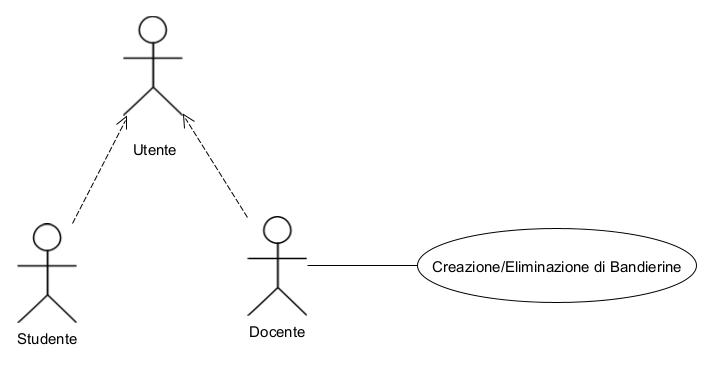
\includegraphics[scale=0.6]{Immagini/EnvironmentInteractionUseCase.jpg}
    \caption{Diagramma dei caso d'uso Creazione/Eliminazione Bandierina}
    \label{fig:my_label}
\end{figure}
\section{Diagrammi Workflow}
La definizione dei casi d'uso porta a scomporre il progetto nelle sue parti costituenti. \\Ognuna di queste risponde ad una specifica necessità emersa dall'analisi dei requisiti. \\Molti casi d'uso si sono tradotti quasi direttamente in un diagramma \textit{workflow}, che mostra il flusso delle diverse attività in un caso d'uso. \\In particolare sono stati definiti 3 diagrammi \textit{workflow} che corrispondono a 3 casi d'uso descritti in precedenza:
\begin{itemize}
   \item Autenticatione Workflow;
   \item Create Room Workflow;
   \item Join Room Workflow.
\end{itemize}
L'analisi di questi 3 casi d'uso, più il caso d'uso \textit{Voice Chat}, verrà poi svolta più dettagliatamente dai colleghi Emanuele Sapio e Lorenzo Iacopetta nelle loro Relazioni, visto che riguarda la parte di cui si sono occupati nel progetto.
\\I rimanenti casi d'uso verranno analizzati dettagliatamente in un capitolo a parte, il \textbf{Cap.4}, per evidenziare meglio la parte del progetto svolta dal sottoscritto.
\subsection{Autenticazione}
\begin{figure}[H]
    \centering
    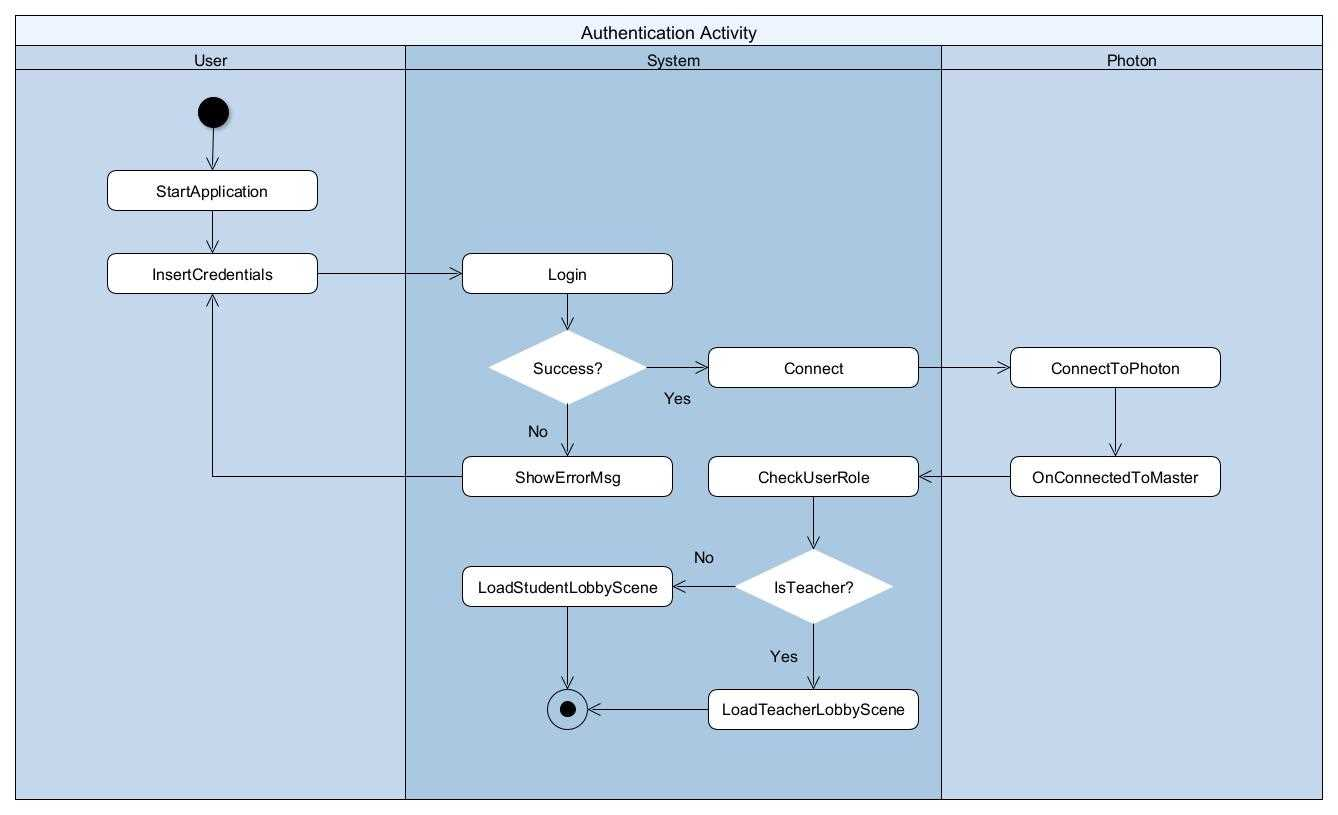
\includegraphics[width = 17cm, height = 14cm]{Immagini/AuthenticationActivityDiagram1.jpg}
    \caption{Diagramma Workflow di Autenticazione}
    \label{fig:my_label}
\end{figure}
L'autenticazione degli utenti ricopre un ruolo importante all'interno dell'applicazione, perché, in base al ruolo dell'attore, il sistema caricherà scene diverse e si avranno diritti e funzioni diverse.
\\Quando l'applicazione viene avviata, il sistema mostrerà all'utente una schermata in cui è possibile inserire le proprie credenziali ed effettuare l'accesso. 
\\In seguito al click dell'attore sul pulsante \textit{Login}, il sistema deve verificare che le credenziali siano corrette. 
\\Se l'utente non esiste nella base dati, il sistema deve restituire un messaggio di errore all'utente che può ripetere l'operazione, altrimenti il sistema si connette ad un server esterno (\textit{server Photon}).
\\Il server Photon possiede un identificativo, nascosto all'utente, che deve essere necessariamente impostato correttamente dal programmatore per poter permettere la comunicazione tra applicazioni diverse (e quindi utenti diversi), perciò le applicazioni con lo stesso identificativo si connetteranno allo stesso server di Photon.
\\In seguito alla connessione al server, il sistema verifica il ruolo dell'utente che si è appena collegato. 
\\Se si tratta di un docente, l'applicazione caricherà la scena dedicata ai docenti che permetterà, oltre ad accedere ad aule già presenti, la creazione di una nuova aula. 
\\Altrimenti, se l'attore è uno studente, il sistema caricherà la scena dedicata agli studenti, in cui è possibile scegliere ed entrare in un'aula.
\\Il flusso termina quando il sistema carica la scena appropriata per l'utente che si è collegato.
\subsection{Create Room}
\begin{figure}[H]
    \centering
    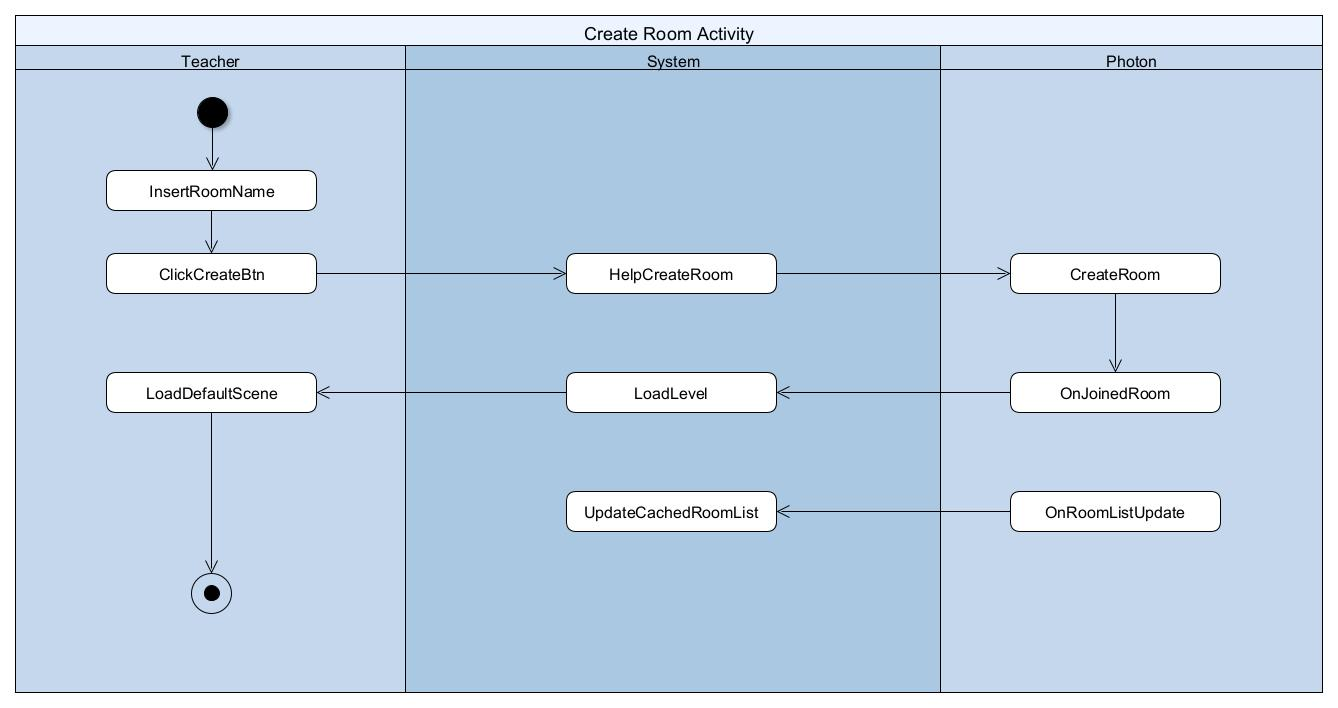
\includegraphics[width = 17cm, height = 13cm]{Immagini/CreateRoomActivityDiagram.jpg}
    \caption{Diagramma Workflow di Create Room}
    \label{fig:my_label}
\end{figure} 
In questo diagramma sono mostrate le attività che vengono svolte durante la creazione della stanza da parte del docente.
\\Il docente, innanzitutto, deve inserire un nome che verrà assegnato all'aula e cliccare sul bottone \textit{Create Room}.
\\Il sistema, a questo punto, invierà la richiesta di creazione di una stanza al server Photon che creerà un'istanza sul proprio server etichettata con il nome che il docente ha assegnato all'aula.
\\Dopodiché, il server Photon aziona una funzione di ingresso, per il docente, alla stanza appena creata, infine il sistema, sull'applicazione del docente, caricherà la scena in cui poi gli utenti andranno ad interagire.
\\La stanza creata dal docente sarà poi visibile a tutti gli altri utenti che accederanno alla scena adibita all'ingresso delle stanze virtuali, grazie all'operazione \textit{OnRoomListUpdate} del server Photon.
\subsection{Join Room}
\begin{figure}[H]
    \centering
    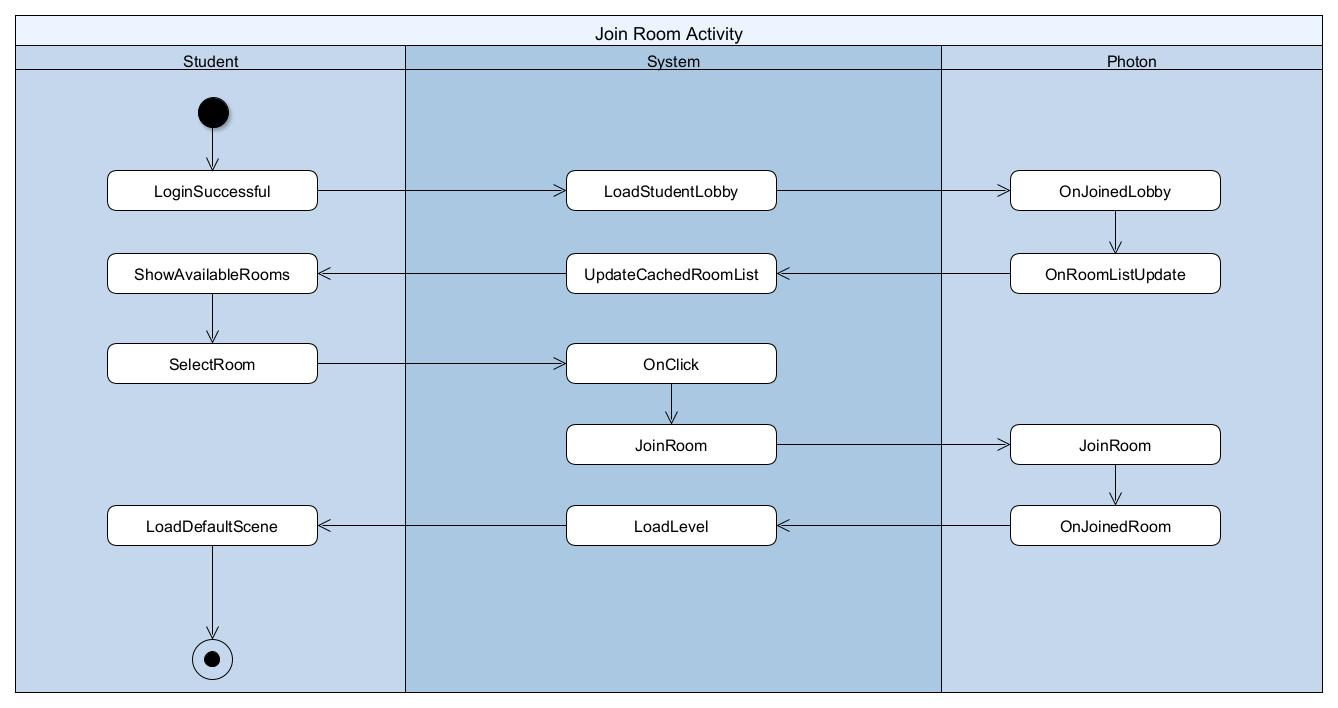
\includegraphics[width = 17cm, height = 13cm]{Immagini/JoinRoomActivityDiagram.jpg}
    \caption{Diagramma Workflow di Autenticazione}
    \label{fig:my_label}
\end{figure}
In questo diagramma sono illustrate le attività svolte durante l'operazione di collegamento ad una stanza creata. 
\\Come già accennato in precedenza, gli studenti visualizzeranno una scena in cui compare solo l'elenco delle aule disponibili, mentre gli insegnanti avranno anche la possibilità di creare una nuova aula. 
\\Come analizzato nel diagramma \textit{workflow} di Create Room, si tratta di una distinzione importante delle attività dell'applicazione rispetto a quelle del server Photon. 
\\L'accesso al server Photon, infatti, è del tutto trasparente all'utente perché è gestito dal server esterno.
\\Il compito del sistema, in questo caso, sarà quello di caricare e mostrare all'utente la lista delle stanze disponibili a cui si può collegare.
\\Una volta caricate le aule disponibili, l'utente può sceglierne una, e al click, l'applicazione invierà la richiesta di ingresso all'aula al server Photon. 
\\Sarà poi il sistema, in seguito all'attività del server, a caricare la scena relativa all'aula selezionata.
\\Quindi, ogni applicazione possiede una o più scene da caricare, quello che permette la comunicazione tra utenti è la connessione allo stesso server Photon.
\\Gli utenti potranno vedersi e interagire tra loro nella scena finale grazie alla presenza di un \textit{avatar}: ogni utente possiede un \textit{avatar} che è stato progettato con delle componenti \textit{sofware} in grado di renderlo percepibile a tutti gli altri utenti collegati alla stessa stanza virtuale.